\chapter*{basic array functions}\addcontentsline{toc}{chapter}{basic array functions}

\hypertarget{arrays}{}

Basic operations, functions or methods which apply on any kind of matrices 
(numerical, strings, arrrays of cells, ...) and sometimes on other 
nsp objects (list, hash table,...).

\HCode{<hr>}
basic array operations

\begin{quote}
\noindent
\hyperlink{indexing arrays}{indexing arrays} - various ways of indexing arrays \\
\hyperlink{sub2ind}{sub2ind} - convert multi-dimensional indexing to linear indexing \\
\hyperlink{ind2sub}{ind2sub} - convert linear indexing to multi-dimensional indexing \\
\hyperlink{dollar}{dollar} - shortcut notation for the last element\\
\hyperlink{extraction assignment deletion}{extraction assignment deletion} - basic array operations\\
\hyperlink{concatenation}{concatenation} - concatenation of matrices\\
\hyperlink{concatr}{concatr} - method, catenate a matrix by another one on the right side\\   
\hyperlink{concatd}{concatd} - method, catenate a matrix by another one on the down side\\   
\hyperlink{set_diag}{set\_diag} - (method) set a diagonal of a matrix \\
\hyperlink{repmat}{repmat} - replicate a matrix\\
\end{quote}


\HCode{<hr>}
sizes, tests, reshape 

\begin{quote}
\noindent
\hyperlink{size}{size} - dimensions of an array, size of some objects \\
\hyperlink{length}{length} - length of an object  \\
\hyperlink{numel}{numel} - length of an object, number of elements of an object  \\
\hyperlink{isvector}{isvector} - vector test\\
\hyperlink{isscalar}{isscalar} - scalar test\\
\hyperlink{isempty}{isempty} - empty matrix or object test\\
\hyperlink{redim}{redim} - reshape a matrix\\
\hyperlink{matrix}{matrix} - reshape a matrix\\
\hyperlink{reshape}{reshape} - reshape a matrix\\
\end{quote}


\HCode{<hr>}
permutations and subsets

\begin{quote}
\noindent
\hyperlink{perms}{perms} - generate all permutations of a vector\\
\hyperlink{nchoosek}{nchoosek} - compute a binomial coefficient or all k-subsets of a set \\
\hyperlink{perm_elem}{perm\_elem} - (method) apply (in place) an elementary permutation to a vector or matrix \\
\end{quote}


% -*- mode: latex -*-

\mansection{indexing arrays, extraction, assignment}
\begin{mandesc}
   \short{indexing arrays}{various ways of indexing arrays}\\
   \short{extraction assignment deletion}{basic array operations}\\
   \short{dollar}{name the last element}\\
\end{mandesc}

\paragraph{Two ways of indexing arrays}
\begin{itemize}

\item  An array element can be adressed using its row 
 and column numbers. For example, the element in row 2
 and column 3 of the array $A$ is retrieved by
 $e = A(2,3)$ (this operation is called {\bf extraction}) 
and changed using $A(2,3) = f$ ({\bf assignment} operation). 
The row  index comes first, followed by the column index. 
Note that currently only two-dimensionnal arrays are available in nsp
(multidimensionnal array should be simulated).
The function \manlink{size}{size} is used to obtain the two dimensions
of any array.

\item A matrix $x$ with only one row is call called a {\bf row vector} 
and a matrix with only one column is called a {\bf column vector}. 
Vector elements are adressed by the preceeding way, but it is more natural
 to use a single indexing, for instance entry 3 in the
 row vector $x$ can be extracted with $e = x(1,3)$ but $e = x(3)$ works. 

\item Note that scalars and vectors are simply bidimensionnal 
arrays with special sizes, $1 \times 1$ for scalars, $1 \times n$ for
row vectors and  $m \times 1$ for columns vectors ; testing if an array
is a vector or a scalar can be done either by the size function
or directly using \manlink{isvector}{isvector} or \manlink{isscalar}{isscalar}
functions. The total number of entries in an array is obtained with
\manlink{numel}{numel} (or \manlink{length}{length} in most cases but
note a special behavior for arrays of strings).


\item An {\bf important feature} is that any matrix can be adressed with
 a single indexing (like in the fortran langage). It is  and called 
``column major order'' as illustrated by the
 following figure:    
$$
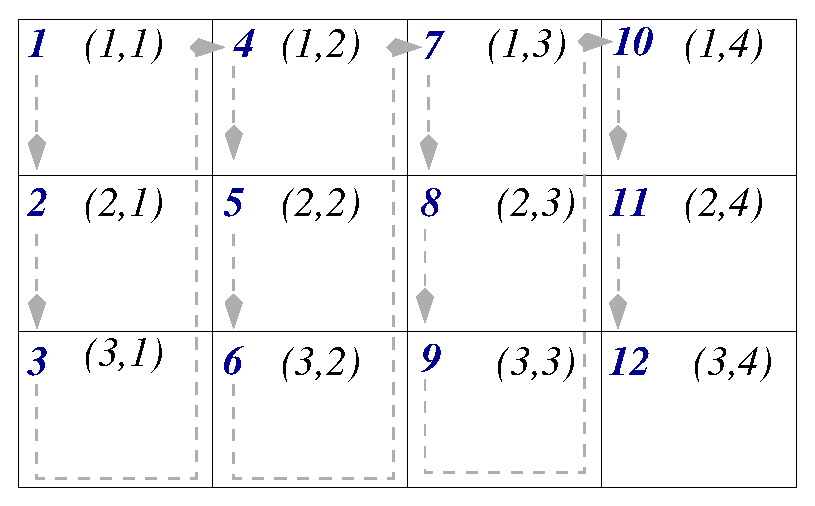
\includegraphics[width=6cm]{indexing} 
$$
The ``column major order'' (in blue) means simply that elements of the first
column are ordered first (from top to bottom) followed by those of
the second column, etc... This way of adressing array will be called
linear indexing. An exemple:
\begin{Verbatim}
A = rand(3,4)
A(2,2) = -2   // usual assignment (to the value -2) of the matrix element in position (2,2)
A(5) = 100    // assignment of the same matrix element (to the value 100) using linear indexing
\end{Verbatim}
Conversion between usual indexing and linear indexing can be done 
using the functions \manlink{sub2ind}{sub2ind}, \manlink{ind2sub}{ind2sub} (see 
also \manlink{ndind2ind}{ndind2ind}).
\end{itemize}

\paragraph{The dollar}

The dollar symbol \verb+$+ is a shortcut to denote:
\begin{itemize}
\item the last index of a vector if linear indexing is used: 
\verb+v($)+ stands for \verb+v(n)+ if the vector $v$ has $n$ elements
or for \verb+v(m*n) = v(m,n)+ if $v$ is an $m \times n$ array.
\item or the last row or column index if the ``two way'' indexing is
used: if $A$ is a $m \times n$ array then \verb+A($,3)+ stands for
\verb+A(m,3)+ and  \verb+A(2,$)+  for \verb+A(2,n)+.
\end{itemize}
Usual arithmetic operations are available with the dollar, for instance
\verb+v($-1)+ corresponds to the last but one vector element.


\paragraph{More on extraction and assignment}

\begin{itemize}
\item Another {\bf important feature} is that sub-vector or sub-matrix
      can be adressed in only one instruction for extraction or assignment:
      \begin{itemize}
      \item If $v$ is a (row or column) vector of length $n$ and  $ind$ a vector 
      of $k$ indices (also called an {\bf index vector}) 
      with values $ind(i)$ between $1$ and $n$ then:
      \begin{Verbatim}
      w = v(ind)
      \end{Verbatim}
      creates a new vector $w$ with $k$ elements such that $w(i) = v(ind(i))$, $1 \le i \le k$.
     Note that the new vector $w$ has row form if $v$ is a row vector
     and has column form otherwise (if $v$ is a column vector but also 
     if $v$ is a matrix and also when $v$ is a scalar and $ind$ an index 
     vector with all its elements equal to 1). The form of the index vector
     (row, column or even matrix) don't play any role in the form
     of $w$. Some examples:
     \begin{Verbatim}
     v = randn(1,6)
     w = v([1,3,5]) // extracts odd elements
     w = v(1:2:6)   // same thing (but with the index vector built using the a:inc:b mechanism)
     w = v(1:2:$)   // same then before but using the dollar symbol in place of its explicit value
     w = v([2,4,6]) // extract even elements
     w = v(2:2:$)   // same thing
     w = v($:-1:1)  // reverse the vector
     w = v([1,1,3,3])
     \end{Verbatim}
 
     \item If $A$ is a matrix of size $m \times n$, $indr$ an index vector of $r$ indices (with values
     between $1$ and $m$) and $indc$ an index vector of $c$ indices (with values between $1$ and $n$)
          then:
     \begin{Verbatim}
         B = A(indr,indc)
     \end{Verbatim}
     creates a new matrix $B$ of size $r \times c$ such that $B(i,j) = A(indr(i),indc(j))$, $1 \le i \le r$
     and $1 \le j \le c$. Some examples:
     \begin{Verbatim}
     A = randn(3,4)
     B = A([1,3],[1,3])
     B = A(2, :)   // extraction of the 2d row (: is a shortcut to denote all the corresponding range)
     B = A(:,3)    // extraction of the 3d column
     B = A([1,2],[4,1])
     \end{Verbatim}
 
     \end{itemize}

\item {\bf assignment} in sub-vector or sub-matrix works the same way, for instance in:
      \begin{Verbatim}
      v(ind) = w
      A(indr,indc) = B
      \end{Verbatim}
      $w$ and $B$ should have (respectively) the same matrix dimensions than what should be obtain with the extractions
      \verb+v(ind)+ and \verb+A(indr,indc)+ but some additionnal features/tricks exist:
      \begin{itemize}
      \item the rhs could be in any case a scalar, and the scalar is assigned to each matrix element denoted by the 
         indexing ;
      \item when the linear indexing is used on a matrix (which is not a vector) the rhs could be either a row
            or column vector ;
      \item the values of the indices could be larger than the matrix dimensions ; {\bf we don't recommand to use
            this rather bad trick} ; special values are used to fill the array where not defined initially 
            (0 for numerical arrays), see examples.
      \end{itemize}
     \begin{Verbatim}
     A = randn(3,4)
     A([1,2],[3,4]) = [-20,30;-30,20]  // usual assignment
     A([1,2],[3,4]) = 0  // the rhs could be a scalar
     A(2,6) = 2   // an example of assignment outside the current matrix dim => enlargement
     \end{Verbatim}
\end{itemize}

\paragraph{Indexing using boolean vectors as index vectors}  

Boolean vectors could be used instead
of numerical ones either for usual indexing or for linear indexing. The convention is simply
that true values are replaced by their corresponding index while false values are not used.
So the boolean vector \verb+[%t, %f, %f, %t, %f, %t]+ is converted as the index vector
\verb+[1, 4, 6]+. The actual usage is for expression like:
\begin{Verbatim}
     x = randn(1,8)
     x( x < 0 ) = 0  // set all negative values to zero
\end{Verbatim}
     

\paragraph{Element, row or column deletion}

Finally it is possible to delete:
\begin{itemize}
\item some elements of a vector using: \verb+x(ind) = []+
\item some rows of a matrix using:\verb+A(ind,:) = []+  
\item some columns of a matrix using:\verb+A(:,ind,:) = []+ 
\end{itemize}
Here \verb+ind+ is an index vector and all corresponding elements/rows/columns are removed.
Some examples:
\begin{Verbatim}
     x = randn(1,9)
     x(x<0) = []  // remove negative values
     A = rand(3,4)
     A(2,:) = []  // remove row 2
     A(:,[1,3]) = []  // remove column 1 and 3
\end{Verbatim}




\begin{manseealso}
    \manlink{size}{size}, \manlink{isvector}{isvector}, \manlink{isscalar}{isscalar}, \manlink{redim}{redim}, \manlink{reshape}{reshape}, \manlink{matrix}{matrix}
\end{manseealso}

% -*- mode: latex -*-

\mansection{sub2ind, ind2sub}
\begin{mandesc}
   \short{sub2ind}{convert multi-dimensional indexing to linear indexing}\\
   \short{ind2sub}{convert linear indexing to multi-dimensional indexing}\\
\end{mandesc}

%-- Calling sequence section
\begin{calling_sequence}
\begin{verbatim}
 // two dimensional indexing <-> linear indexing
 Ind = sub2ind(dims, I, J)
 Ind = sub2ind(dims, I, J, ind_type=str)
 [I,J] = ind2sub(dims, Ind)
 [I,J] = ind2sub(dims, Ind, ind_type=str)

 // multi-dimensional indexing <-> linear indexing
 Ind = sub2ind(ndims, I1, I2, ..., In)
 Ind = sub2ind(ndims, I1, I2, ..., In, ind_type=str)
 [I1,...,In] = ind2sub(ndims, Ind)
 [I1,...,In] = ind2sub(ndims, Ind, ind_type=str)
\end{verbatim}
\end{calling_sequence}

%-- Parameters
\begin{parameters}
  \begin{varlist}
   \vname{dims}: vector with the 2 dimensions of a two-dimensional array.
   \vname{I,J}: vectors of indices of same size.
   \vname{ndims}: vector with the n dimensions of a n-dimensional array.
   \vname{I1,...,In}: vectors of indices of same size.
   \vname{Ind}: vector of indices.
   \vname{ind_type=str}: named optional, str can be equal to \verb"double" (default) in which case
          the resulting indices are stored as double floating point numbers or equal to  \verb"int"
          to be stored as int32 numbers.
  \end{varlist}
\end{parameters}

\begin{mandescription}
This function lets to convert between linear indexing and two-dimensional indexing
(see \manlink{indexing arrays}{indexing arrays} to understand the various
ways of indexing arrays). It can be also used for conversion between linear
indexing and multi-dimensional indexing. 

\itemdesc{linear $\leftrightarrow$ two-dimensional indexing conversions}

Denoting by $m$ the number of rows and $n$ the number of columns of a matrix, 
a two dimensional index is a couple $(i,j)$ with $1 \le i \le m$ and
$1 \le j \le n$ and corresponds to the linear index $k = (j-1) \times m + i$
with $1 \le k \le m \times n$ (see \manlink{indexing arrays}{indexing arrays} 
about the various ways of indexing arrays). 

Given the vector \verb+dims = [m,n]+ and $p$ such couples $(i,j)$ under the form 
of two vectors \verb+I+ and \verb+J+ each with $p$ components \verb+Ind=sub2ind(dims,I,J)+
computes the $p$ corresponding linear index and given \verb+dims+ and \verb+Ind+
\verb+[I,J]=ind2sub(dims,Ind)+ do the inverse operation.

\itemdesc{linear  $\leftrightarrow$ multi-dimensional indexing conversions}

The same conversion can be done for multi-dimensional arrays (even if nsp
doesn't yet support arrays with more than 2 dimensions). Considering a $n$
dimensional arrays with dimensions $m_1 \times m_2 \times \dots \times m_n$,
a nd-index is a $n$-tuple $(i_1,i_2,\dots, i_n)$ with $1 \le i_k \le m_k$
for $k=1,\dots,n$ and corresponds to the linear index:
$$
   k = i_1 + m_1 \left( i_2-1 + m_2 \left( i_3 - 1 + m_3 \left( \dots \right) \right) \right)  
$$ 

In this case \verb+dims=[m1,m2,...,mn]+ and the conversion can be done between $p$ such $n$-tuple
under the form of $n$ vectors \verb+I1+, \dots, \verb+IN+ with $p$ components each one, and 
the vector \verb+Ind+ with $p$ components with the corresponding linear indices.    

\itemdesc{named optional arg ind\_type}

Output indices vector(s) can be stored with doubles float number by default or using \verb+ind_type="double"+
or with 32 bits integer using \verb+ind_type="int"+.

\end{mandescription}

%--example 
\begin{examples}
\begin{mintednsp}{nsp}
// this is the example of the indexing help page
Ind = sub2ind([3,4],2,2)   // should be 5
[I,J] = ind2sub([3,4],5)   // should be 2 and 2

// how to add fastly 1 to the diagonal of a matrix
A = rand(5,5)
Ind = sub2ind([5,5],1:5,1:5);
// now add 1 on the diagonal of A
A(Ind) = A(Ind) + 1
\end{mintednsp}
\end{examples}


%-- see also
\begin{manseealso}
\manlink{indexing arrays}{indexing arrays}
\end{manseealso}


% -*- mode: latex -*-

\mansection{concatenation of matrices}
\begin{mandesc}
   \short{concatenation}{concatenation of matrices}\\
   \short{concatr}{method, catenate a matrix by another one on the right side}\\   
   \short{concatd}{method, catenate a matrix by another one on the down side}\\   
\end{mandesc}

%-- Calling sequence section
\begin{calling_sequence}
\begin{verbatim}
 C = [A , B]  // right concatenation (a new matrix is build)
 A.concatr[B] // right concatenation, matrix A is modified
 C = [A ; B]  // down concatenation (a new matrix is build)
 A.concatd[B] // down concatenation, matrix A is modified
\end{verbatim}
\end{calling_sequence}

%-- Parameters
\begin{parameters}
  \begin{varlist}
   \vname{A, B, C}: matrices (of numbers, strings, cells,...)
  \end{varlist}
\end{parameters}

\begin{mandescription}
\begin{itemize}
\item The right concatenation involves two (or more) matrices having the same number of rows
      and build a new matrix by stacking the second matrix at the right of the first one.
      With $A$ of size $m \times n_A$ and $B$ of size $m \times n_B$, one gets
      with \verb+C = [A , B]+ a new matrix of size $m \times (n_A + n_B)$. The method 
      form \verb+A.concatr[B]+ is a efficient shortcut for  \verb+A = [A , B]+.
\item The down concatenation involves two (or more) matrices having the same number of columns
      and build a new matrix by stacking the second matrix at the bottom of the first one, etc...
      With $A$ of size $m_A \times n$ and $B$ of size $m_B \times n$, one gets
      with \verb+C = [A ; B]+ a new matrix of size $(m_A + m_B) \times n$. The method form 
      \verb+A.concatd[B]+ is a efficient shortcut for  \verb+A=[A ; B]+.
\item Right and dow concatenations may be combined in various natural ways to build a matrix
      from smaller blocks, see examples.
\end{itemize}

\end{mandescription}

%--example 
\begin{examples}

\begin{Verbatim}
// a first matrix build by several right concatenations and one down concatenation 
A = [1,2,3;4,5,6]
// another one
B = [-1, -2; -3, -4]
// right concatenation of A and B
C = [A, B]
// in place right concatenation of A by B
A.concatr[B]
A

// a more complicated concatenation
A11 = eye(2,2)
A12 = rand(2,3)
A2 = randn(1,5)
A3 = ones(3,1)
A = [ [A11, A12; A2] , A3 ]
\end{Verbatim}


\end{examples}


%-- see also
\begin{manseealso}
\manlink{extraction assignment deletion}{extraction assignment deletion}, \manlink{repmat}{repmat}
\end{manseealso}

\mansection{set\_diag}
\begin{mandesc}
  \short{set_diag}{set a diagonal of a matrix}
\end{mandesc}
%-- Calling sequence section
\begin{calling_sequence}
\begin{verbatim}
  A.set_diag[v]
  A.set_diag[v,k]
\end{verbatim}
\end{calling_sequence}
%-- Parameters
\begin{parameters}
  \begin{varlist}
    \vname{A}: any kind of matrix
    \vname{v}: vector or scalar (of same type than A)
    \vname{k}: optional argument, the diagonal number (default is $0$)
  \end{varlist}
\end{parameters}

\begin{mandescription}

  This function sets the given diagonal $k$ (0 by default) of a matrix 
with either a vector (which must have as many elements as the given 
diagonal) or with a scalar (the given diagonal is filled with the
scalar).

Remarks:  
\begin{itemize}
\item The matrix element $A_{i,j}$ is located on the diagonal number $j-i$. So main 
diagonal is numbered $0$, the diagonal number $1$ and $-1$ are respectively located just 
upper and under the main diagonal, etc...
  $$
  \includegraphics[width=8cm]{diagonal} 
  $$

\item For a sparse matrix, argument $v$ can be given also using a full vector (or scalar).

\end{itemize}

\end{mandescription}

%--example 
\begin{examples}
\begin{Verbatim}
A = zeros(5,5)
A.set_diag[2]; A.set_diag[-1,1];  A.set_diag[-1,-1]; 
print(A)

// same example with a sparse matrix
A = sp_create(5,5)
A.set_diag[2]; A.set_diag[-1,1];  A.set_diag[-1,-1]; 
print(A)

// an example with a IMat
A = imat_create(4,6)
for k=-3:5; A.set_diag[m2i(k),k]; end
print(A)

// an example with a string matrix
A = smat_create(3,3)
A.set_diag["a",-2]
A.set_diag[["b","c"],-1]; 
A.set_diag[["d","e","f"],0]; 
A.set_diag[["g","h"],1]; 
A.set_diag[["i"],2]; 
print(A)
\end{Verbatim}
\end{examples}

%-- see also
\begin{manseealso}
  \manlink{diag}{diag}, \manlink{tril}{tril}, \manlink{triu}{triu}
\end{manseealso}


% -*- mode: latex -*-

\mansection{size}
\begin{mandesc}
  \short{size}{dimensions of an array, size of some objects}
\end{mandesc}
% -- Calling sequence section
\begin{calling_sequence}
\begin{verbatim}
dims = size(A)
[m,n] = size(A)
m = size(A,1)  // or m = size(A,"r")
n = size(A,2)  // or m = size(A,"c")
mn = size(A,0) // or m = size(A,"*")   
\end{verbatim}
\end{calling_sequence}

% -- Parameters
\begin{parameters}
  \begin{varlist}
    \vname{A}: matrix
    \vname{dims}:  row vector (\verb+1x2+) of integers
    \vname{m, n, mn}: integers
  \end{varlist}
\end{parameters}

\begin{mandescription}
\verb+size+ gives the dimensions of an array with the following features:
\begin{itemize}
  \item \verb!dims = size(A)! (that is a call with one output argument) returns the matrix dimensions in a row vector 
        (the first element is the number of rows $m$, the second the number of columns $n$) ;
  \item \verb![m,n] = size(A)! (a call with 2 output arguments) returns the number of rows $m$ in the first output arg
        and the number of columns $n$ in the second output arg.
  \item \verb!m = size(A,1)! (or equivalently \verb!m = size(A,"r")! returns the number of rows
  \item \verb!n = size(A,2)! (or equivalently \verb!n = size(A,"c")! returns the number of columns
  \item \verb!n = size(A,0)! (or equivalently \verb!n = size(A,"*")! returns the product of the dimensions (this is
        also equivalent to \manlink{numel}{numel}).
\end{itemize}

Note also that like \manlink{numel}{numel} and \manlink{length}{length}, if \verb+L+ is a list, 
\verb+size(L)+ returns the number of its elements, and if \verb+H+ is an hash table \verb+size(H)+ 
returns the number of its entries.
\end{mandescription}

\begin{examples}
\begin{Verbatim}
A = rand(3,4)
dims = size(A)
[m,n] = size(A)
size(A,1)
size(A,2)
size(A,"*")

// for list and hash tables, size behaves like length and numel
L = list(1,2); L(5)=78; 
size(L)
length(L)
numel(L)

H = hcreate(A=9,B=%t);
size(H)
length(H)
numel(H)
\end{Verbatim}
\end{examples}

% -- see also
\begin{manseealso}
  \manlink{numel}{numel}, \manlink{length}{length} 
\end{manseealso}


% -*- mode: latex -*-

\mansection{length}
\begin{mandesc}
  \short{length}{length of object}
\end{mandesc}
% -- Calling sequence section
\begin{calling_sequence}
\begin{verbatim}
n=length(M)   
\end{verbatim}
\end{calling_sequence}

% -- Parameters
\begin{parameters}
  \begin{varlist}
    \vname{M} : an object.
    \vname{n} : integer or integer matrix
  \end{varlist}
\end{parameters}

\begin{mandescription}
\begin{itemize}
  \item  For all type of matrices  except string matrices, \verb!length(M)! is equal to \verb!size(M,'*')!  number of columns of \verb!M!.
  \item For a string matrix \verb+M+, \verb+n=length(M)+ returns a numerical matrix \verb+n+ such that 
    \verb+n(i,j)+ is the string length of string \verb+M(i,j)+.
  \item For \verb+M+ of type list, the function returns the index of the last list entry in list \verb+M+.
\end{itemize}
\end{mandescription}

\begin{examples}
  \begin{program}
    length(string(rand(3,4)))
    L = list(1,2); L(5)=78; length(L)
    length(rand(5,7))
  \end{program}
\end{examples}

% -- see also
\begin{manseealso}
  \manlink{size}{size}  
\end{manseealso}


% -*- mode: latex -*-

\mansection{repmat}
\begin{mandesc}
   \short{repmat}{replicate a matrix}
\end{mandesc}

%-- Calling sequence section
\begin{calling_sequence}
\begin{verbatim}
 B = repmat(A,m,n)
\end{verbatim}
\end{calling_sequence}

%-- Parameters
\begin{parameters}
  \begin{varlist}
   \vname{A}: matrix (of numbers, strings, cells,...)
   \vname{m,n}: non negative integers
  \end{varlist}
\end{parameters}

\begin{mandescription}
  Build the matrix $B$ by replicating the matrix $A$ in $m$ row blocs and $n$ column blocs :
$$
 B=
     \begin{array}{cc}
             \begin{array}{ccccc} 1 & \hdots & \hdots & \hdots & n \end{array}  &          \\
      \left[ \begin{array}{ccccc} A     & A       & \hdots & \hdots & A     \\
                                     A     & A       & \hdots & \hdots & A     \\
                                    \vdots & \vdots  &   .    &    .    & \vdots\\
                                     A     & A       & \hdots & \hdots  & A 
                \end{array} \right] &
      \begin{array}{c} 1 \\ \vdots \\ \vdots \\ m \end{array}
     \end{array}
$$ 

If the matrix $A$ is $m_A \times n_A$ the matrix $B$ is  $ m m_A \times n n_A$.

\end{mandescription}

%--example 
\begin{examples}

\paragraph{simple examples}
\begin{Verbatim}
A = [1,2,3;4,5,6]
repmat(A,4,3)

A = ["a", "ab", "abc"]
repmat(A,3,2)
\end{Verbatim}

\paragraph{computing distance between a set of points in 3d space}

In the following an array $dist$ is build where $dist(i,j)$ is the 
euclidian distance between points $i$ and $j$.
\begin{Verbatim}
n = 6;
P = randn(3,n);
Xp = P(1,:); Yp = P(2,:); Zp = P(3,:);
Dx = repmat(Xp,n,1) - repmat(Xp',1,n);
Dy = repmat(Yp,n,1) - repmat(Yp',1,n);
Dz = repmat(Zp,n,1) - repmat(Zp',1,n);
dist = sqrt( Dx.^2 + Dy.^2 + Dz.^2)
\end{Verbatim}

\end{examples}


%-- see also
\begin{manseealso}
\manlink{ones}{ones}, \manlink{concatenation}{concatenation}
\end{manseealso}

% -*- mode: latex -*-

\mansection{perms}
\begin{mandesc}
   \short{perms}{generate all permutations of a vector}
\end{mandesc}

%-- Calling sequence section
\begin{calling_sequence}
\begin{verbatim}
 p = perms(v)
\end{verbatim}
\end{calling_sequence}

%-- Parameters
\begin{parameters}
  \begin{varlist}
   \vname{v} : vector (of numbers, strings, cells,...)
   \vname{p} : matrix of size $n! \times n$ if $n$ is the number of
               elements of $v$.
  \end{varlist}
\end{parameters}

\begin{mandescription}
  Computes all permutations of a vector: each row of $p$
  corresponds to a permutation of $v$. 

\paragraph{remark}
This function don't currenly work for $n > 10$ because of memory
needs ($11! = 39\,916\,800$).

\end{mandescription}

%--example 
\begin{examples}
\begin{program}\HCode{p=perms(1:4)\Hnewline
p = perms(["biniou","grand-mere","gratte"])}
\end{program}
\end{examples}


%-- see also
%\begin{manseealso}
%\manlink{factor}{factor}
%\end{manseealso}

%-- Author
\begin{authors}
B. Pincon
\end{authors}


% -*- mode: latex -*-

\mansection{nchoosek}
\begin{mandesc}
   \short{nchoosek}{compute a binomial coefficient or all k-subsets of a set}
\end{mandesc}

%-- Calling sequence section
\begin{calling_sequence}
\begin{verbatim}
 cnk = nchoosek(n,k)  // first form
 Ek = nchoosek(E,k)   // second form
\end{verbatim}
\end{calling_sequence}

%-- Parameters
\begin{parameters}
  \begin{varlist}
   \vname{n}: non negative integer scalar
   \vname{E}: vector (of numbers, strings, cells,...) with at least 2 elements (if $E$ reduces to a 
              scalar then the first form is considered)
   \vname{k}: non negative integer scalar less or equal to $n$ or to the number of elements of $E$
   \vname{cnk}: binomial coefficient
   \vname{Ek}: matrix with all k-subsets elements of $E$
  \end{varlist}
\end{parameters}

\begin{mandescription}
  This function has two differents behaviors depending of the size of the first argument:
\begin{enumerate}
\item if it is a scalar it should be a non negative integer and the binomial coefficient :
$$
  \left( \begin{array}{c} n \\ k \end{array} \right) = \frac{n!}{k!(n-k)!} =  \left( \begin{array}{c} n \\ n-k \end{array} \right)
$$
is computed.
\item if it is not a scalar then all the subsets with $k$ elements of the vector $E$ are computed
      (it is supposed that all components of $E$ are unique) ; $Ek$ should have 
      $ \left( \begin{array}{c} n \\ k \end{array} \right)$ rows and $k$ columns, each
      row corresponding to a subset.
\end{enumerate}

\end{mandescription}

%--example 
\begin{examples}
\paragraph{first form examples}
\begin{Verbatim}
nchoosek(6,4)

// should be equal to 6!/(4!*2!) and n! could be computed by prod(1:n)
prod(1:6)/(prod(1:4)*prod(1:2))

// test symmetry
nchoosek(6,2)
\end{Verbatim}
\end{examples}

\begin{examples}
\paragraph{second form}
\begin{Verbatim}
// all subsets with 3 elements of {1,2,3,4,5}
nchoosek(1:5,3)

// all subsets with 2 elements of {"biniou","grand-mere","gratte"}
nchoosek(["biniou","grand-mere","gratte"],2)
\end{Verbatim}
\end{examples}


%-- see also
\begin{manseealso}
\manlink{perms}{perms}
\end{manseealso}

%-- Author
\begin{authors}
F. Delebecque, B. Pincon
\end{authors}


% -*- mode: latex -*-

\mansection{perm\_elem}
\begin{mandesc}
   \shortunder{perm\_elem}{perm_elem}{(method) apply in place an elementary permutation to a vector or matrix}
\end{mandesc}

%-- Calling sequence section
\begin{calling_sequence}
\begin{verbatim}
 M.perm_elem[p,q[,dim]]
\end{verbatim}
\end{calling_sequence}

%-- Parameters
\begin{parameters}
  \begin{varlist}
   \vname{M}: vector or matrix (of numbers, strings, cells,...)
   \vname{p, q}: integer scalars.
   \vname{dim}: optional, an integer scalar among $\{0,1,2\}$, default is 0.
  \end{varlist}
\end{parameters}

\begin{mandescription}
Depending on the parameter dim, this method permutes in place:  
\begin{itemize}
\item when {\bf dim = 0}, the $p$ and $q$ elements (if $M$ is a matrix
 the element numbering comes from the column  major order).
\item when {\bf dim = 1}, the $p$ and $q$ rows.
\item when {\bf dim = 2}, the $p$ and $q$ columns.
\end{itemize}

\end{mandescription}

%--example 
\begin{examples}
\begin{Verbatim}
A = [ "abc", "de",  "fg" ]
A.perm_elem[1,3]
A

B = randn(3,4)
B.perm_elem[2,4,2]  // permute columns 2 and 4
B

B = randn(3,4)
B.perm_elem[1,3,1]  // permute rows 1 and 3
B

B = randn(2,3)
B.perm_elem[1,4]  // permute elements 1 and 4 (so B(1,1) and B(2,2))
B
\end{Verbatim}
\end{examples}


%-- see also
\begin{manseealso}
\manlink{perms}{perms}
\end{manseealso}

%-- Author
\begin{authors}
B. Pincon
\end{authors}


% -*- mode: latex -*-

\mansection{redim, matrix}
\begin{mandesc}
  \short{redim}{reshape a matrix in place (method)} \\
  \short{matrix}{reshape a matrix}
\end{mandesc}
% -- Calling sequence section
\begin{calling_sequence}
\begin{verbatim}
A.redim[mm, nn]
A.redim[newdims]

B = matrix(A,mm, nn)
B = matrix(A,ndims)
\end{verbatim}
\end{calling_sequence}

% -- Parameters
\begin{parameters}
  \begin{varlist}
    \vname{A}: matrix
    \vname{ndims}:  vector made of 2 integers
    \vname{mm, nn}: integers
  \end{varlist}
\end{parameters}

\begin{mandescription}
\verb+redim+ and \verb+matrix+ lets to reshape of matrix $A$ with dimensions
$m \times n$ as a matrix of sizes $mm \times nn$ such that 
$mm \times nn = m \times n$ (that is they have the same number of elements).
The internal ``one dimensionnal'' order of the elements matrix are not changed
(column major order). 

\verb+redim+ is a method and work in place.

For both:
\begin{itemize}
  \item the new dimensions could be provided either as 2 scalar integer arguments or as a vector with 2 integers.
  \item if you want to reshape the matrix as a row vector you can use \verb+-1+ as second dimension number (this
        avoid to remember or ask how many elements the matrix has) and equivalently you can specify \verb+-1+ as 
        first dimension to reshape the matrix as a column vector, so:
        \begin{verbatim}
        A.redim[1,-1]  // reshape A in place as a row vector
        B = matrix(A,1,-1) // the same with matrix
        A.redim[-1,1]  // reshape A in place as a column vector
        B = matrix(A,-1,1) // the same with matrix
        \end{verbatim}
\end{itemize}

\end{mandescription}

\begin{examples}
\begin{Verbatim}
A = rand(3,4)
A.redim[2,6]; A
A.redim[-1,1]; A

B = matrix(A,1,-1)
B = matrix(A,6,2)
\end{Verbatim}
\end{examples}

% -- see also
\begin{manseealso}
   \manlink{size}{size}, \manlink{numel}{numel}, \manlink{length}{length} 
\end{manseealso}


% -*- mode: latex -*-

\mansection{basic array or object structure tests}
\begin{mandesc}
  \short{isvector}{vector test} \\
  \short{isscalar}{scalar test} \\
  \short{isempty}{empty matrix or object test}
\end{mandesc}
% -- Calling sequence section
\begin{calling_sequence}
\begin{verbatim}
b = isvector(A)
b = isscalar(Obj)
b = isempty(Obj)
\end{verbatim}
\end{calling_sequence}

% -- Parameters
\begin{parameters}
  \begin{varlist}
    \vname{A}: matrix of any kind
    \vname{Obj}: any nsp object (matrix of any kind, list, hash table,...)
    \vname{b}:  boolean scalar
  \end{varlist}
\end{parameters}

\begin{mandescription}
\begin{itemize}
\item \verb+isvector+ tests if a matrix is a vector that is if one of its 2 dimensions is equal to 1. 
      Note that empty matrices of size $0 \times 1$ and $1 \times 0$ are detected as vectors.
\item \verb+isscalar+ tests if a matrix is a scalar that is if it is of size $1 \times 1$.
      \verb+isscalar+ also applies on lists and hash tables and returns true if they contains only
      one element or one entry.
\item \verb+isempty+ tests if an object is empty, that is if it is a matrix of size $0 \times n$ or $m \times 0$ or
      if it is an empty list, or an hash table with no entries.
\end{itemize}

If you want to test if a matrix of some kind/type is a vector or scalar you should combine
several tests for instance:
\begin{verbatim}
   is(A,%types.Mat") && isvector(A)               // test if a numerical (full) matrix is a vector
   type(A,"string") == "Mat" && isvector(A)       // same test but using the type function

   is(A,%types.Mat") && isvector(A) && isreal(A)   // test if a numerical (full) matrix is a real vector

   is(A,%types.Mat") && isscalar(A) && isreal(A)   // test if A is a real scalar

   is(A,%types.SMat") && isscalar(A)               // test if A is a (scalar) string
\end{verbatim}

If you want to test the row or column form of a vector, use \manlink{size}{size} instead of \verb+isvector+:
\begin{verbatim}
   is(A,%types.Mat") && size(A,1)==1 && isreal(A)       // test if a numerical (full) matrix is a real row vector

   is(A,%types.Mat") && size(A,2)==1 && isreal(A)       // test if a numerical (full) matrix is a real column vector

   is(A,%types.SpColMat") && size(A,2)==1 && isreal(A)  // test if a sparse matrix is a real (sparse) column vector
\end{verbatim}

\end{mandescription}

\begin{examples}
\begin{Verbatim}
A = randn(3,1)
isvector(A)
iscalar(A)

B = zeros(1,0)
isempty(B)     // should return true
isvector(B)    // should return true
\end{Verbatim}
\end{examples}

% -- see also
\begin{manseealso}
   \manlink{size}{size}, \manlink{numel}{numel}, \manlink{length}{length}, \manlink{is}{is}, \manlink{type}{type} 
\end{manseealso}


